\chapter{Conceção}
\label{chap:Chapter4}
\tbd
% Neste capítulo apresenta-se a abordagem conceptualizada e parcialmente implementada no protótipo. O objetivo é oferecer uma visão da solução a alto nível e ir explorando os seus detalhes. Assim sendo, na Secção~\ref{sec:chap04_general_vision} descreve-se a solução na sua globalidade, dando ênfase à arquitetura de sistema e à descrição de cada componente. Posteriormente, na Secção~\ref{sec:chap04_conception}, descrevem-se os aspetos relevantes da conceção, incluindo o processo de trabalho usado ao longo desta fase, os requisitos identificados, a análise e desenho do sistema. Na Secção~\ref{sec:chap04_development} expõem-se os pormenores de desenvolvimento do protótipo considerados relevantes e, por fim, na Secção~\ref{sec:chap04_validation} apresentam-se os tópicos de validação, cujos resultados obtidos serão pertinentes para a conclusão da presente tese.

%%%%%%%%%%%%%%%%%%%%%%%%%%%%%%%%%
%           SECTION
%%%%%%%%%%%%%%%%%%%%%%%%%%%%%%%%%
\section{Análise Exploratória}
\label{sec:chap03_approaches}
Com o propósito de colocar em prática o estudo levado a cabo até este ponto, decidiu-se fazer experimentações envolvendo algumas abordagens e ferramentas apresentadas nas secções anteriores. Posto isto, optou-se por desenvolver pequenas provas de conceito, num período bem definido, de forma a fazer uma rápida avaliação das abordagens, técnicas e ferramentas usadas. Para cada uma, é abordado em que consiste, algumas observações pertinentes e referência dos pontos favoráveis e desfavoráveis.

\subsection{Gramática Baseada em Semântica}
Como proposto em~\textcite[p.~361-403]{natural_language_processing_with_python}, o uso do NLTK permite o desenvolvimento de gramáticas que possibilitam a análise de uma frase pela sua semântica, tal como o exemplo demonstrado a seguir.

\begin{lstlisting}[language=Python,caption={Excerto de uma gramática extraída de~\textcite{natural_language_processing_with_python}},numbers=none,label=lst:grammarexample,basicstyle=\scriptsize]
S[SEM=(?np + WHERE + ?vp)] -> NP[SEM=?np] VP[SEM=?vp]
VP[SEM=(?v + ?pp)] -> IV[SEM=?v] PP[SEM=?pp]
VP[SEM=(?v + ?ap)] -> IV[SEM=?v] AP[SEM=?ap]
NP[SEM=(?det + ?n)] -> Det[SEM=?det] N[SEM=?n]
PP[SEM=(?p + ?np)] -> P[SEM=?p] NP[SEM=?np]
AP[SEM=?pp] -> A[SEM=?a] PP[SEM=?pp]
NP[SEM='Country="greece"'] -> 'Greece'
NP[SEM='Country="china"'] -> 'China'
Det[SEM='SELECT'] -> 'Which' | 'What'
N[SEM='City FROM city_table'] -> 'cities'
IV[SEM=''] -> 'are'
A[SEM=''] -> 'located'
P[SEM=''] -> 'in'
\end{lstlisting}

O código apresentado em~\ref{lst:grammarexample}, usando o NLTK, para a pergunta \inquotes{What cities are located in China?} permite gerar a seguinte \textit{query} de \gls{sql}: SELECT City FROM city\_table WHERE Country=\inquotes{china}. Com esta metodologia é possível mapear diretamente linguagem natural em \gls{sql}, sendo que a gramática funciona como a base de conhecimento. Por conseguinte, torna-se viável a codificação de um \textit{parser} que usa as gramáticas definidas, verificando
alguma é capaz de dar resposta à \textit{query} de linguagem natural.

\subsubsection*{Pontos Favoráveis}
\begin{itemize}
    \item 
    {
        Viabilidade de desenvolvimento de uma solução customizada;
    }
    \item
    {
        Utilização de ferramenta \textit{open source};
    }
    \item 
    {
        Tradução imediata de linguagem natural para \gls{sql}. 
    }
\end{itemize}

\subsubsection*{Pontos Desfavoráveis}
\begin{itemize}
    \item 
    {
        Dificuldade em criar ou estender gramáticas;
    }
    \item
    {
        Complexidade em adaptar para múltiplas línguas ou domínios;
    }
    \item
    {
        Necessidade de conhecimento linguístico, por forma a adaptar a gramática às regras de uma determinada língua;
    }
    \item
    {
        Ambiguidade da semântica. Diferentes expressões podem ou devem gerar o mesmo \gls{sql};
    }
    \item
    {
        Manutenção difícil.
    }
\end{itemize}

\subsection{Pesquisa Semântica}
Nesta abordagem foi usada uma \textit{framework} que não consta nas ferramentas apresentadas na Secção~\ref{sec:chap03_existingtools}, principalmente porque o seu desenvolvimento encontra-se estagnado desde 2013. Ainda assim, é aceitável o seu uso para testar esta mesma abordagem, no ponto de vista prático. O Quepy é desenvolvido em \textit{Python} e tem como objetivo a transformação de linguagem natural em \textit{SPARQL Protocol and RDF Query Language} (SPARQL)\footnote{Disponível em \url{https://www.w3.org/TR/rdf-sparql-query/}.} e \textit{Metaweb Query Language} (MQL)\footnote{Disponível em \url{https://github.com/nchah/freebase-mql}.}, linguagens de \textit{query} usadas com tecnologia \gls{rdf}\footnote{Disponível em \url{https://www.w3.org/RDF/}.}, \inquotes{um modelo padrão para permuta de dados na Web}\footnote{Tradução livre do autor. No original \inquotes{is a standard model for data interchange on the Web.}.}, intrinsecamente ligado ao campo da Web Semântica~\parencite{resource_description_framework}.

Neste caso, o uso do Quepy implica a definição da linguagem específica de domínio através de código \textit{Python}, respeitando as restrições colocadas na documentação da \textit{framework}, de maneira a que esta seja capaz de reconhecer o padrão introduzido.

\begin{lstlisting}[language=python, caption={Excerto da definição semântica da frase que lida com listagem de produtos},numbers=none,label=lst:quepyexample,basicstyle=\scriptsize]
from quepy.dsl import FixedType, FixedRelation
from quepy.parsing import Lemma, QuestionTemplate

class NameOf(FixedRelation):
    "Name of the entity's property"
    relation = "product_name"
    reverse = True

class IsProduct(FixedType):
    "Defines the entity's type"
    fixedtype = "product"

class ListProducts(QuestionTemplate):
    "Questions such as 'List products' or 'Listing products'"
    regex = Lemma("list") + Lemma("product")

    def interpret(self, match):
        product = IsProduct()
        name = NameOf(product)
        return name, "enum"

\end{lstlisting}

No excerto demonstrado anteriormente em~\ref{lst:quepyexample}, define-se a expressão regular que caracteriza a questão esperada, para além de detalhes relacionados com a linguagem específica de domínio. A \textit{query} obtida pode ser posteriormente usada numa base de dados \gls{rdf}, como o objetivo de recolher os dados. De notar que, neste caso, sendo o propósito a consulta de uma base de dados relacional, seria necessária uma forma de a transpor ou replicar numa camada compatível com tecnologia \gls{rdf}. Para isso, existem ferramentas capazes de executar esse mapeamento, como por exemplo o D2RQ\footnote{Disponível em \url{http://d2rq.org/}.}.

\subsubsection*{Pontos Favoráveis}
\begin{itemize}
    \item
    {
        Viabilidade de desenvolvimento de uma solução customizada;
    }
    \item
    {
        Tecnologia \textit{open source};
    }
    \item 
    {
        Linguagem específica de domínio permite abstração aos detalhes de implementação associados ao reconhecimento de linguagem natural;
    }
    \item
    {
        Reconhecimento da linguagem natural é feita através da análise de expressões regulares, o que torna fácil compreender a estrutura frásica;
    }
    \item
    {
        Transformação da linguagem natural numa representação que obedece à especificação da tecnologia \gls{rdf}, definida pela W3C.
    }
\end{itemize}

\subsubsection*{Pontos Desfavoráveis}
\begin{itemize}
    \item
    {
        As regras de domínio e o modelo de dados devem ser definidos diretamente no código, não possibilitando a extensibilidade por configuração;
    }
    \item
    {
        Rigidez da linguagem usada, já que o uso de expressões regulares implica uma estrutura minimamente estática para que o reconhecimento seja bem sucedido;
    }
    \item
    {
        O uso de tecnologias \gls{rdf} levam a uma nova camada aplicacional, que envolve o uso de ferramentas não relacionadas com o \gls{pln} e que leva a mais esforço na manutenção do sistema;
    }
    \item
    {
        Necessidade de estudo aprofundado ou conhecimento pericial na área de Web Semântica.
    }
\end{itemize}

\subsection{Reconhecimento de Intenções e Entidades}
Neste contexto, foi utilizado o Microsoft LUIS, já descrito na Secção~\ref{sec:chap03_existingtools}. A razão para esta escolha deve-se principalmente a dois fatores: o facto de ser uma das plataformas mais usadas e documentadas, e pela Microsoft disponibilizar este tipo de ferramentas a quem possua subscrição de estudante.

Para esta prova de conceito criou-se um \textit{chatbot} capaz de responder a algumas perguntas colocadas pelo utilizador (\textit{utterance}), identificando qual a sua intenção (\textit{intent}) e quais as entidades envolvidas (\textit{entity}), descritas de seguida, na Tabela~\ref{tab:luis_intents}.

\begin{table}[!ht]
\caption{Descrição de algumas das intenções e entidades dada a expressão de exemplo, baseado em~\textcite[Concepts]{microsoft_luis_official}}
\label{tab:luis_intents}
\centering
\resizebox{\textwidth}{!}{
\renewcommand{\arraystretch}{1.3}
\footnotesize
\begin{tabular}{l*{2}{|l}}
%
\toprule
%
\tabhead{Expressão de Exemplo}&\tabhead{Intenção}&\tabhead{Entidades}\\
%
\midrule
%
{Good Morning}&{Greeting}&{--}\\
%
{What's the weather like in \underline{Porto}?}&{CheckWeather}&{Place}\\
%
{Turn on the Internet in my \underline{bedroom}, please}&{HomeAutomation}&{Room}\\
%
{Book me a flight to \underline{Lisbon} \underline{next week}}&{BookFlight}&{Place, Datetime}\\
%
\bottomrule
%
\end{tabular}
}
\end{table}

O \textit{chatbot} recorre ao Microsoft LUIS para identificar a intenção do utilizador, e com base nisso e nas entidades recolhidas, pode carregar os dados necessários e apresentá-los da forma que for mais adequada. Neste caso, o \textit{chatbot} retorna apenas a intenção que foi capaz de identificar (Figura~\ref{fig:chatbotexample}).

\begin{figure}[!ht]
\centering
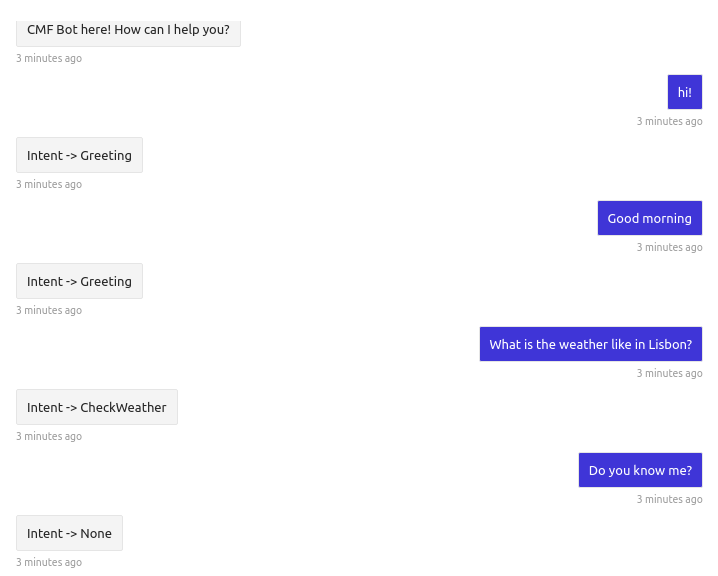
\includegraphics[width=.9\textwidth]{ch03/assets/chatbot.png}
\caption{Resultado do teste com \textit{chatbot} desenvolvido usando Microsoft LUIS}
\label{fig:chatbotexample}
\end{figure}

É possível dotar o \textit{chatbot} de comportamento para manipular os metadados obtidos, e assim, obter dados de uma base de dados relacional ou obter dados estáticos dum serviço de respostas pré-fabricadas, tal como o QnA Maker\footnote{Disponível em \url{https://www.qnamaker.ai/}}. É importante frisar que, embora esta abordagem tenha sido aplicada recorrendo a um \textit{chatbot}, por imposição da própria plataforma, tal não é obrigatório na utilização da mesma numa solução customizada. 

\subsubsection*{Pontos Favoráveis}
\begin{itemize}
    \item
    {
        As plataformas disponíveis na \textit{cloud} constituem um ponto de partida para uma solução personalizada;
    }
    \item
    {
        A solução é fácil de desenvolver, estender e integrar;
    }
    \item
    {
        A base de conhecimento pode ser totalmente configurável;
    }
    \item
    {
        Robustez na identificação de intenções e entidades, através do uso de modelos de \gls{ml};
    }
\end{itemize}

\subsubsection*{Pontos Desfavoráveis}
\begin{itemize}
    \item
    {
        A aplicação desta abordagem numa biblioteca customizada implica o estudo teórico de \gls{ml} aplicado ao \gls{pln} e consequentemente, maior esforço de desenvolvimento;
    }
    \item
    {
        A adição de novas intenções à base de conhecimento leva também à adição de comportamento para lidar com os mesmas.
    }
\end{itemize}

\subsection{Sinopse}
As abordagens descritas anteriormente baseiam-se nas observações e experiências realizadas, no ponto de vista prático. Portanto, a conclusão aqui exposta leva em consideração os pontos favoráveis e desfavoráveis de cada uma.

De uma forma geral, a abordagem que parece a mais adequada é a que diz respeito ao reconhecimento de intenções e entidades, principalmente pela facilidade de compreensão e aplicação do conceito. Além do mais, os pontos desfavoráveis mencionados são de índole operacional, pelo que podem ser superados ou até descartados aquando a conceção e/ou desenvolvimento da solução final. Relativamente às abordagens descartadas, aponta-se que a primeira -- gramática baseada em semântica -- se usada no contexto de uma solução final, será difícil manter o seu desenvolvimento e capacidade de cobrir uma gama aceitável de questões válidas. Já a segunda -- pesquisa semântica --, ainda que assente sobre uma tecnologia especificada e aprovada pelo W3C, necessita de uma camada adicional (\gls{rdf}), contribuindo assim para o aumento do esforço em configuração e manutenção do sistema. Por isso, a terceira abordagem revela-se a mais adequada e será contemplada no protótipo a desenvolver.

%%%%%%%%%%%%%%%%%%%%%%%%%%%%%%%%%
%           SECTION
%%%%%%%%%%%%%%%%%%%%%%%%%%%%%%%%%
\section{Modelo Proposto}
\label{sec:chap04_proposal}
\tbd

\subsection{Visão}
\tbd

\subsection{Casos de Uso}
\tbd

\subsection{Arquitetura}
\tbd

\label{sec:chap04_general_vision}
O objetivo deste trabalho assenta na formulação de uma abordagem capaz de lidar com linguagem natural. Como tal, no capítulo anterior, identificaram-se os casos de estudo, ferramentas e abordagens, cujo estudo contribuiu para o desenho da abordagem aqui apresentada. Pretende-se expor a solução numa perspetiva lógica, partindo do pressuposto que será a abordagem usada no contexto da solução final. Portanto, apresenta-se na Figura~\ref{fig:prototype_architecture} a arquitetura da solução como um todo e o do elemento principal, explicando a responsabilidade inerente a cada componente.

\begin{figure}[!h]
\centering
    \begin{subfigure}{\textwidth}
         \centering
         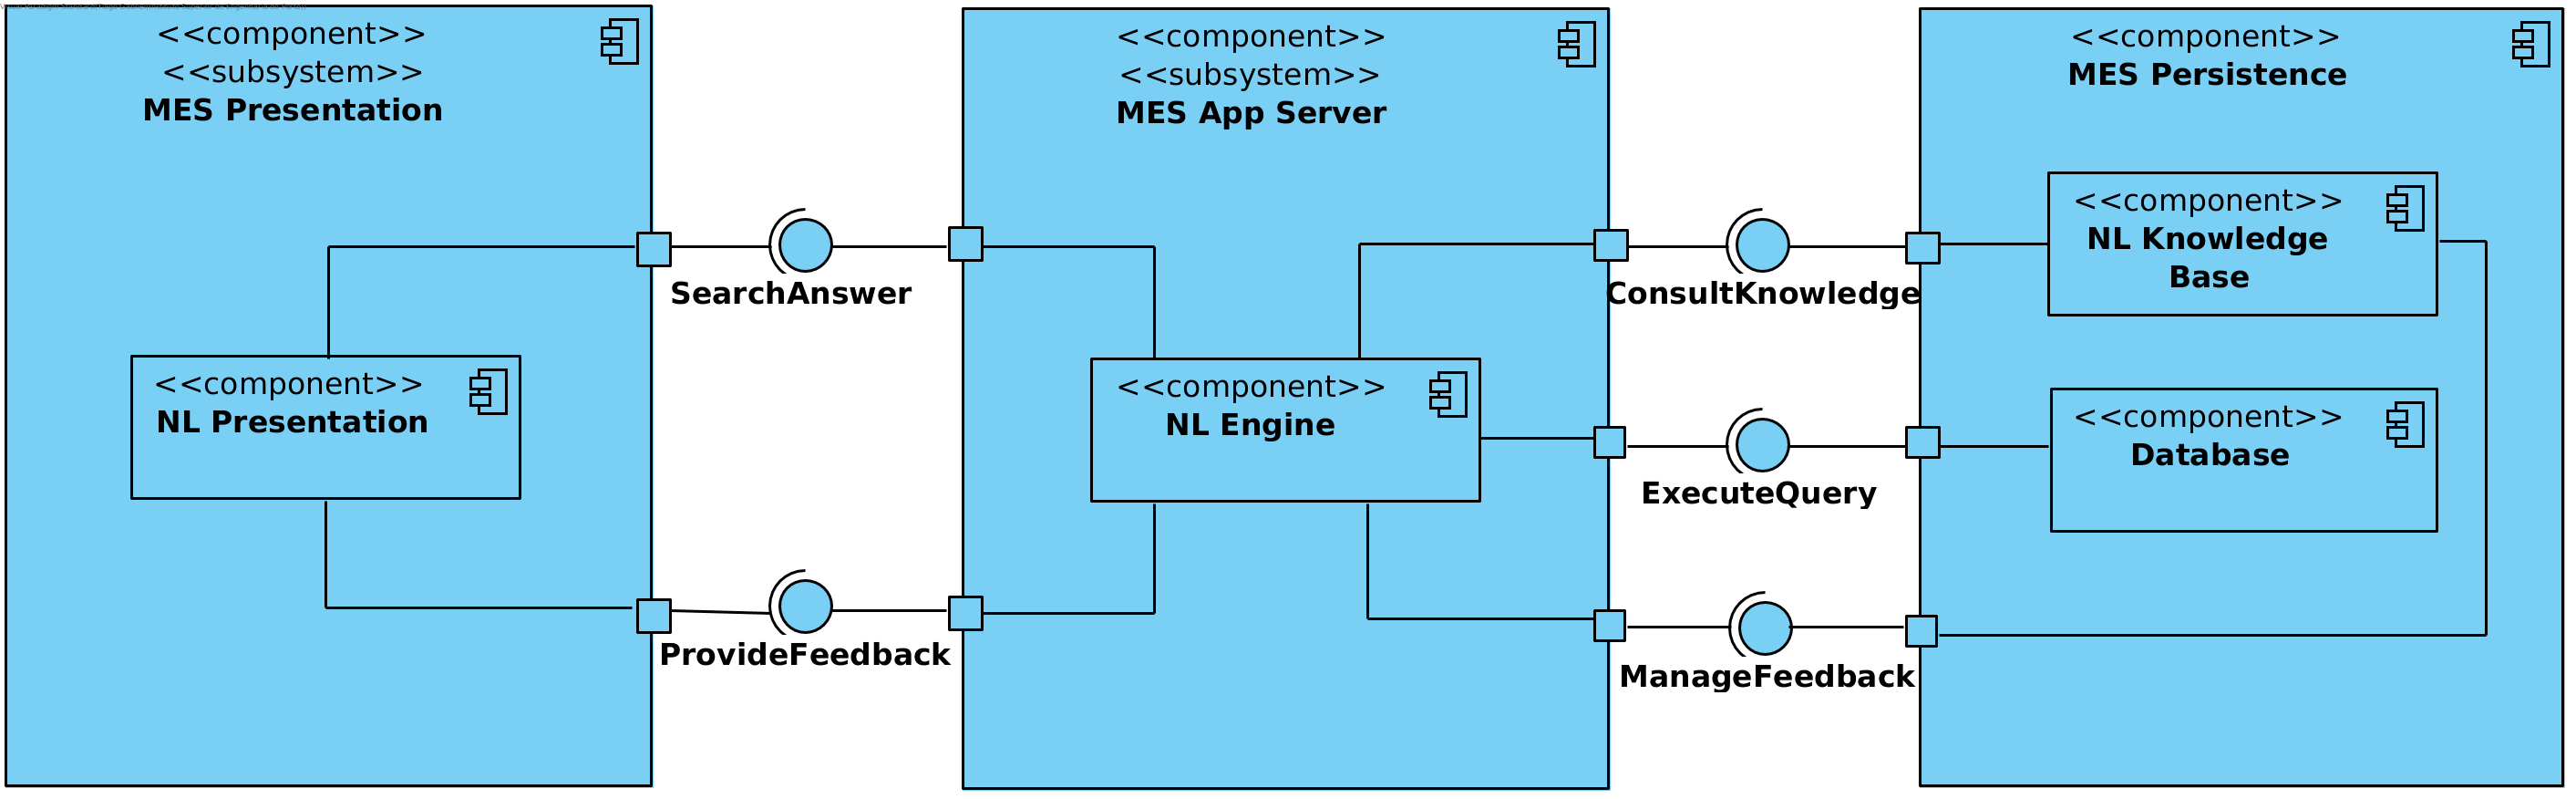
\includegraphics[width=\textwidth]{ch04/assets/architecture.png}
         \caption{Arquitetura genérica do protótipo}
         \label{fig:generic_architecture}
     \end{subfigure}
     \bigbreak
     \bigbreak
     \begin{subfigure}{\textwidth}
         \centering
         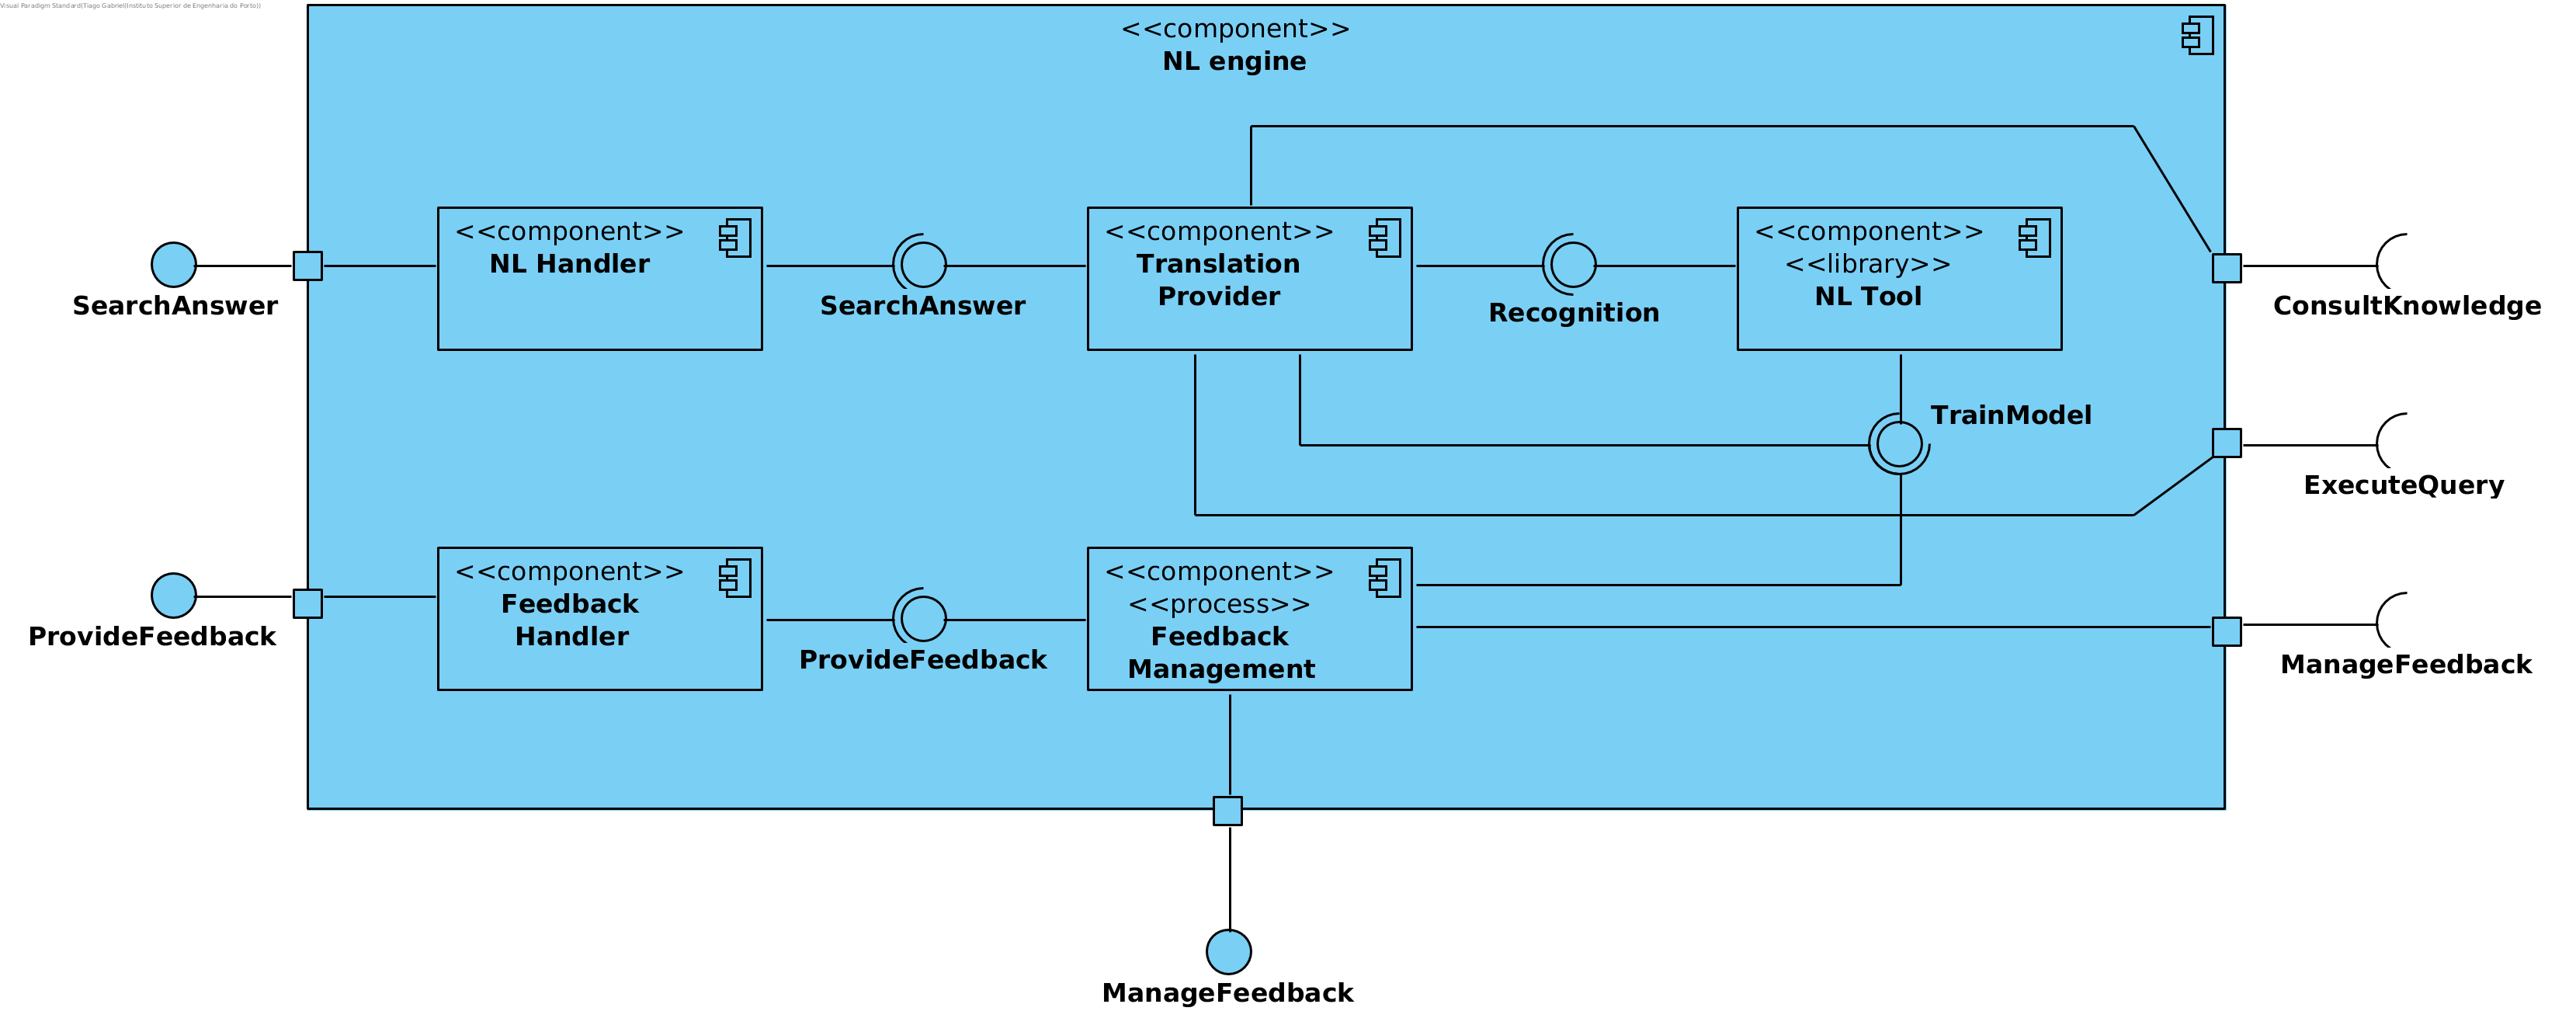
\includegraphics[width=\textwidth]{ch04/assets/nl-engine.png}
         \caption{Arquitetura detalhada do \textit{NL Engine}}
         \label{fig:nlengine_architecture}
     \end{subfigure}
\caption{Arquitetura do protótipo, apresentando um vista genérica e uma mais específica do componente \textit{NL Engine}}
\label{fig:prototype_architecture}
\end{figure}

\begin{itemize}
    \item 
    {
        \textit{NL Presentation} -- responsável pela interação com o utilizador. Integra a camada de apresentação do {\productname} e, como tal, é desenvolvido de acordo com as especificidades do subsistema em que se insere;
    }
    \item 
    {
        \textit{NL Engine} -- o módulo de linguagem natural, ou seja, o \inquotes{motor} que permite a tradução de linguagem natural em intenções e respetivas entidades. Integra a camada aplicacional de serviços do produto;
    }
    \item 
    {
        \textit{NL Handler} -- trata-se de um subcomponente o \textit{NL Engine}, que conhece as partes envolvidas no processo de tradução, sendo responsável orquestrar esse processo. Numa analogia à anatomia humana, pode ser considerado o \inquotes{cérebro} do processo de tradução;
    }
    \item
    {
        \textit{Feedback Handler} -- outro subcomponente de \textit{NL Engine}. Tem a responsabilidade de lidar com o \textit{feedback} providenciado pelo utilizador e disponibiliza serviços para a gestão dessa mesma informação, que incluem o desencadear do processo de aprendizagem, por exemplo;
    }
    \item 
    {
        \textit{Translation Provider} -- também subcomponente do \textit{NL Engine}, trabalha em conjunto com o \textit{NL Tool} e com a base de conhecimento definida (\textit{NL Knowledge Base}) com o objetivo de identificar a intenção e entidades de uma dada \textit{query} de linguagem natural;
    }
    \item 
    {
        \textit{NL Tool} -- a ferramenta escolhida para o \gls{pln};
    }
    \item 
    {
        \textit{Feedback Management} -- processo responsável pela gestão de \textit{feedback} dado ao sistema. Inicialmente, o \textit{feedback} pode ser consultado manualmente, possibilitando o uso dessa informação para a melhoria do sistema. Contudo, podem ser aplicadas estratégias que façam uso desta informação de forma automática;
    }
    \item 
    {
        \textit{NL Knowledge Base} -- base de conhecimento de domínio, incluída na camada de persistência do {\productname}. É configurada pela equipa de desenvolvimento e deve mapear as entidades de domínio, as intenções em que estão envolvidas e suportar o registo de \textit{feedback}, para que possa ser usado na aprendizagem do módulo;
    }
    \item 
    {
        \textit{Database} -- armazém de dados de negócio. Contém a informação que o utilizador deseja obter através de linguagem natural.
    }
\end{itemize}

Apesar da elucidação acerca da responsabilidade de cada componente no sistema, é importante detalhar a forma como estes interagem entre si, para atingir o objetivo. A Figura~\ref{fig:prototype_sequence_diagram} mostra como se desenrola a comunicação entre os diversos componentes, que se passa a descrever: \textit{descreve-se o workflow}

\begin{sidewaysfigure}
    \centering
    
\includegraphics[width=\textwidth]{no-image.png}
    \caption{Comunicação entre os componentes do módulo de linguagem natural}
    \label{fig:prototype_sequence_diagram}
\end{sidewaysfigure}

%%%%%%%%%%%%%%%%%%%%%%%%%%%%%%%%%
%           SECTION
%%%%%%%%%%%%%%%%%%%%%%%%%%%%%%%%%
\section{Síntese do Capítulo} 
\label{sec:chap04_chaptersummary}
\tbd
